\documentclass[12pt]{article}
\usepackage[hmargin=2.0cm,vmargin=1cm]{geometry}
\usepackage[utf8]{inputenc}
\usepackage{graphicx}
\usepackage{float}
\usepackage{natbib}
\usepackage{amsmath}

\title{\begin{LARGE}
{HW2 ISM, Radiative transfer and processes}
\end{LARGE}}

\author{Juan Nicol\'as Garavito Camargo}

\begin{document}
\maketitle


\begin{LARGE}
\textbf{1.}
\end{LARGE}

If the source function can be approximated as: 

\begin{equation}\label{approx}
S(\tau) \approx S(\tau_{*}) + S'(\tau_*)(\tau - \tau_*) + \dfrac{1}{2}S''(\tau_*)(\tau-\tau_*)^2	
\end{equation}

Then the full general solution of the radiative transfer equation 
for the emergent intensity can be writen as:

\begin{equation}\label{sol}
I_{\nu}(\tau_1, \mu) = I_{\nu}(\tau_2, \mu) e^{-(\tau_2 - \tau_1)/\mu} + \dfrac{1}{\mu}\int_{\tau_1}^{\tau_2}S_{\nu}(\tau ')e^{-(\tau ' - \tau_1)/\mu} d\tau '
\end{equation}

Now replacing the approximated source function we get:


\begin{equation}
I_{\nu}(\tau_1, \mu) = I_{\nu}(\tau_2, \mu) e^{-(\tau_2 - \tau_1)/\mu} + 
\dfrac{1}{\mu} \int_{\tau_1}^{\tau_2} e^{-(\tau ' - \tau_1)/\mu} d\tau ' 
\left[  S(\tau_{*}) + S'(\tau_*)(\tau ' - \tau_*) + \dfrac{1}{2}S''(\tau_*)(\tau '-\tau_*)^2 \right] d\tau '
\end{equation}

Now I treat these 3 integrals separately:\\

The first integral involving the term $S(\tau_*)$ is:

\begin{equation}\label{int1}
\int_{\tau_1}^{\tau_2}e^{-(\tau ' - \tau_1)/\mu} S(\tau_*) d\tau ' =
S(\tau_*)\int_{\tau_1}^{\tau_2}e^{-(\tau' - \tau_1)/\mu} d\tau ' = S(\tau_*) (-\mu) \left[ e^{-(\tau_2 - \tau_1)/\mu} - 1 \right]
\end{equation}

The second integral corresponding to the $S'(\tau_*)$ term is:

\begin{equation*}
\int_{\tau_1}^{\tau_2}e^{-(\tau ' - \tau_1)/\mu} S'(\tau_*)(\tau ' - \tau_*) d\tau ' = S'(\tau_*) \int_{\tau_1}^{\tau_2}e^{-(\tau ' - \tau_1)/\mu} (\tau ' - \tau_*)
d\tau ' = -\mu S'(\tau_*)(\mu - \tau_* + \tau')e^{-(\tau ' - \tau_1)/\mu}
\end{equation*}

\begin{equation}\label{int2}
= -\mu S'(\tau_*)\left[ (\mu - \tau_* + \tau_2)e^{-(\tau_2 - \tau_1)/\mu} - (\mu - \tau_* + \tau_1) \right]
\end{equation}


Finally the third integral correspoding to the $S''(\tau_*)$ term is:

\begin{equation*}
\dfrac{1}{2}\int_{\tau_1}^{\tau_2}e^{-(\tau ' - \tau_1)/\mu} S''(\tau_*)(\tau ' - \tau_*)^2 d\tau' = \dfrac{S''(\tau_*)}{2} \int_{\tau_1}^{\tau_2}e^{-(\tau ' - \tau_1)/\mu} (\tau ' - \tau_*)^2 d\tau'  
\end{equation*}

\begin{equation*}
 =  \dfrac{S''(\tau_*)}{2} \left[-\mu (\tau_{*}^2 - 2\tau_*(\mu+\tau') + 2\mu^2 + 2\mu \tau' + \tau'^2)e^{-(\tau'-\tau_1)/{\mu}} \right]
\end{equation*}

\begin{equation}\label{int3}
= \dfrac{-\mu S''(\tau_*)}{2} \left[ (\tau_{*}^2 - 2\tau_*(\mu+\tau_2) + 2\mu^2 + 2\mu \tau_2 + \tau_{2}^2)e^{-(\tau_2 -\tau_1)/{\mu}} - (\tau_{*}^2 - 2\tau_*(\mu+\tau_1) + 2\mu^2 + 2\mu \tau_1+ \tau_{1}^2) \right]
\end{equation}

If $\tau_* = \mu$ and $\tau_1 = 0$ the terms that would be affected are Eq.\ref{int2} \& Eq.\ref{int3}
correspondly.

\begin{equation}
 = -\mu S'(\tau_*)\left[ \tau_2 e^{-(\tau_2-\tau_1)/\mu} - \tau_1\right] = -\mu S'(\tau_*) \tau_2 e^{-\tau_2/\mu} \approx 0
\end{equation}

Note that we assume here that $\tau_2 >>1$.

\begin{equation}
= \dfrac{-\mu S''(\tau_*)}{2} \left[ (\mu^2 + \tau_{2}^2)e^{-(\tau_2 -\tau_1)/{\mu}} - (\mu^2 + \tau_{1}^2) \right] = \dfrac{-\mu S''(\tau_*)}{2} ( -\mu^2 ) = \dfrac{\mu^3 S''(\tau_*)}{2}
\end{equation}


\begin{LARGE}
\textbf{2.}
\end{LARGE}

If we are in LTE then our source function is that of a Black 
Body,  the general solution of the emergent intensity as we demonstrated
in class is:

\begin{equation}
I_{\nu} = I_{\nu}(0)e^{-\tau_{\nu}} + B_{\nu}(T)\left[ 1 - e^{-\tau_{\nu}} \right]
\end{equation}

If we are observing the source trough the nebula the emergent intensity would be:

\begin{equation}\label{I1}
I_{\nu, 1 } = I_{\nu}(T_s)e^{-\tau_{\nu}} + I_{\nu}(T_n)\left[ 1 - e^{-\tau_{\nu}} \right]
\end{equation}

Now if we are not in the line of sight of the source function the emergent
intensity would be:

\begin{equation}\label{I2}
I_{\nu, 2} = I_{\nu}(T_n)\left[ 1 - e^{-\tau_{\nu}} \right]
\end{equation}

Then we can infer the optical depth of the Nebula from the above two 
equations if we substract Eq.\ref{I1} \& Eq.\ref{I2}:

\begin{equation}
I_{\nu, 1} - I_{\nu, 2} = I_{\nu}(T_s)e^{-\tau_{\nu}}
\end{equation}

To finaly get:

\begin{equation}
\tau_{\nu} = -Ln \left( \dfrac{I_{\nu, 1} - I_{\nu, 2}}{I_{\nu}(T_s)}  \right)
\end{equation}

Now in the Rayleigh Jeans limit: 

\begin{equation}
I_{\nu}^{RJ} (T_s) = \dfrac{2\nu^2}{c^2}KT_s
\end{equation}

Which let us derive the optical depth:

\begin{equation}
\tau_{\nu} = -Ln \left( \dfrac{c^2(I_{\nu, 1} - I_{\nu, 2})}{2\nu^2 KT_s}  \right)
\end{equation}



\begin{LARGE}
\textbf{3.}
\end{LARGE}

\begin{figure}
\centering
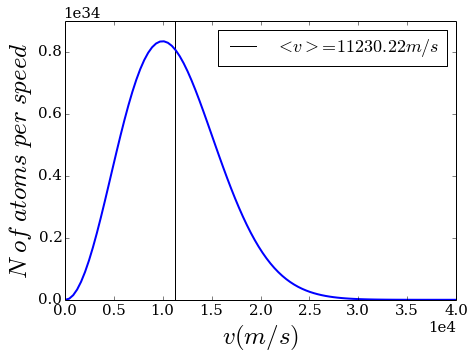
\includegraphics[scale=0.5]{mbv.png}
\caption{Velocity distribution for $10^{38}$Hydrogen atoms 
in the solar photosphere\label{mbv}}
\end{figure}

1. \\
Figure \ref{mbv} show the velocity distribution of thw $10^{38}$ atoms
in the solar photosphere. The black vertical line shows the typical
speed of a Hydrogen atom, which was computed as follows:

\begin{equation}
<v> = 2\int_0^{\infty} \left( \dfrac{m}{2\pi KT}  \right)^{3/2} 4\pi v^3 e^{-mv^2/KT}
\end{equation}

\begin{equation}
<v> = 8\pi \left( \dfrac{m}{2\pi KT}  \right)^{3/2} \left(\dfrac{KT}{m}\right)^4
= 2 \left( \dfrac{2}{\pi} \right)^{1/2} \left( \dfrac{KT}{m}  \right)^{1/2}
\end{equation}

\begin{equation}
<v> = 11203.22 \dfrac{m}{s}
\end{equation}

2. \\ 

The number of photons (N1) within a 1\% of $<v>$ can be computed with the CDF as follows:


\begin{equation}
N1 = erf(v/\sqrt{2}a) - \sqrt{\dfrac{2}{\pi}} \dfrac{v e^{-v^2/2a^2}}{a} \Bigg|_{0.99<v>}^{1.01<v>}  = 9.07\times 10^{35} 
\end{equation}

3. \\

The Doppler shifht due to the speed $<v>$ would be:

\begin{equation}
\dfrac{\nu}{\nu_0} = (1 + <v>/c) =  1.000037
\end{equation}

4. \\ 

The velocity that would produce a doppler shift twice as the previous
is:

\begin{equation}
v2 = 22406.44 \dfrac{m}{s}
\end{equation} 

And the number of photons that would be within the $1\%$ 
of $v2$ are:

\begin{equation}
N2 = erf(2v/\sqrt{2}a) - \sqrt{\dfrac{2}{\pi}} \dfrac{2v e^{-v^2/a^2}}{a} \Bigg|_{0.99<2v>}^{1.01<2v>}  = 6.48\times 10^{35} 
\end{equation}

5.\\

And finally for a doppler shift fourth times:

\begin{equation}
v4 = 44812.88 \dfrac{m}{s}
\end{equation}

And the number of photons that would be within the $1\%$
of $v4$ are:

\begin{equation}
N4 = erf(4v/\sqrt{2}a) - \sqrt{\dfrac{2}{\pi}} \dfrac{4v e^{-2v^2/a^2}}{a} \Bigg|_{0.99<4v>}^{1.01<4v>}  = 2.56\times 10^{35} 
\end{equation}

This number is roughly three times less than the one that we obtain in part 2. 


\begin{LARGE}
\textbf{4.}
\end{LARGE}

a.\\

To show that $h \nu << KT$ for HII regions we select the extreme case that
corresponds to $\lambda = 1mm$. Using the fact the typical temperature 
of a HII region is $10^4$K we found that: 

\begin{equation}
h \nu = 1.98 \times 10 ^{28} J
\end{equation} 

\begin{equation}
KT_{HII} = 1.38 \times 10^{-19} J
\end{equation}

b.\\

Then for radio observations it is valid to work in the Rayleigh-Jeans limit.
If it is the case we can expressed the Intentisy in terms of the brigthness 
temperature as follows:

\begin{equation}
B_{\nu}(T) = \dfrac{2\nu^2}{c^2}KT
\end{equation}

\begin{equation}
T_b = \dfrac{c^2}{2\nu^2K}I_{\nu}
\end{equation}

\begin{equation}
I_{\nu} = T_{\nu} (0)  e^{-\tau_{\nu}} + B_{\nu}(T)(1- e^{-\tau_{\nu}})
\end{equation}

\begin{equation}
\dfrac{2 \nu^2 K}{c^2} T_{\nu} = \dfrac{2 \nu K}{c^2}T_b(0)e^{-\tau_{\nu}} + \dfrac{2 \nu^2 K}{c^2} T(1 - e^{-\tau_{\nu}})
\end{equation}

\begin{equation}\label{T}
T_{b} = T_b (0)  e^{-\tau_{\nu}} + T(1- e^{-\tau_{\nu}}) 
\end{equation}

c.\\

Eq.(15.29) of the text says that:

\begin{equation}\label{1529}
\rho \kappa_{\nu}^{ff} = \sum_{i} n(Z_i) n_e \left( \dfrac{2m_e}{3\pi K T} \right)
\left[ \dfrac{4 \pi Z_i^2 e^6}{3 m_e^2 c h \nu^3} \right] \bar{g}_{ff}(\nu) 
\left( 1 - e^{-h\nu / KT}\right)
\end{equation}

For  $h \nu << KT$ that we have already shown that it is the case for the radio
wavelengths we can expand the last term in Eq.\ref{1529} as:

\begin{equation}\label{aprox}
\left( 1 - e^{-h\nu / KT}\right) \approx 1 - \left(1 - \dfrac{h \nu}{KT} \right)
= \dfrac{h \nu}{KT}
\end{equation}
  

Now we can express Eq.\ref{1529} as:

\begin{equation}\label{rhok}
\rho \kappa_{\nu}^{ff} = \sum_{i} n(Z_i) n_e \left( \dfrac{2m_e}{3\pi K T} \right)
\left[ \dfrac{4 \pi Z_i^2 e^6}{3 m_e^2 c h \nu^3} \right] \bar{g}_{ff}(\nu)\dfrac{h \nu}{KT}
\end{equation}

And using the definition of the C constant as:

\begin{equation}
C = \left( \dfrac{2m_e}{3\pi KT} \right)^{1/2} \left[ \dfrac{4\pi e^6}{3m_e^2 cK} \right]
\end{equation}

Then Eq.\ref{rhok} can be expressed as:

\begin{equation}
\rho \kappa_{\nu}^{ff} = \sum_{i} n(Z_i) n_e C Z_i^2 T^{-3/2} \nu^{-2} bar{g}_{ff}(\nu)
\end{equation}

And for a pure Hydrogen plasma $Z_i = 1$ and $\sum_{i}n(Z_1)=n_e$ we found the 
following expression: 

\begin{equation}
\rho \kappa_{\nu}^{ff} =  n_e^2 C T^{-3/2} \nu^{-2} \bar{g}_{ff}(\nu)
\end{equation}

d.\\

The Gaunt factor $\bar{g}_{ff}(\nu)$ for in the radio regime is computed using:

\begin{equation}
\bar{g}_{ff}(\nu) = \dfrac{\sqrt{3}}{2\pi} \left[
ln\left( \dfrac{8K^3T^3}{\pi^2 e^4 m_{e} \nu^2} 
- 5 \gamma \right) \right]
\end{equation}

We compute the Gaunt factor using the following values:

\begin{itemize}
\item $\gamma = 0.5772$
\item $T=10^4 K$ 
\item $\nu = 10^{9}Hz$
\item $K = 1.38e-23 J/K$
\item $m_e = 9.10e-31 Kg$
\item $e = 4.8e-10 Fr$

\end{itemize}

With these values we get:

\begin{equation}
\bar{g}_{ff}(\nu) = 5.96
\end{equation}

e.\\ 

Now using the definition of EM:

\begin{equation}
EM = \int n_e^2 ds
\end{equation}

The optical depth can de expressed as:

\begin{equation}
\tau_{\nu} = \int \rho \kappa_{\nu}^{ff} ds = 
\int C n_e^2 T^{-3/2}\nu^{-2}bar{g}_{ff}(\nu)
=  C T^{-3/2}\nu^{-2}\bar{g}_{ff}(\nu) \int n_e^2 ds 
= C T^{-3/2}\nu^{-2}\bar{g}_{ff}(\nu) (EM)
\end{equation}

f.\\

Now at low frequencies when $\tau_{\nu}>>1$ and without background source $T_b$
from Eq.\ref{T} can be expressed as: 

\begin{equation}
T_b = T(1-e^{-\tau_{\nu}}) = T(1 - 0) = T
\end{equation}


While for low frequencies $\tau_{\nu}<<1$ $T_b$ can be expressed as:

\begin{equation}
T_b = T(1-e^{-\tau_{\nu}}) = T(1 -(1- \tau_{\nu})) = T\tau_{\nu}
\end{equation}

g.\\

The flux can be simply approximated by the Intrinsic intensity $I_{\nu}$
per solid angle that for a distant espherical source can be approzimated 
as $\pi R_s^2$ where $R_s$ is the radius of the source, and divided per 
the distance $r$ squared of the source. Then:

\begin{equation}
F_{\nu} = \pi I_{\nu} \left( \dfrac{R_s^2}{r^2}\right) 
\end{equation}
 
h.\\

Wich in temrs of the brightness temperature can be expressed as:

\begin{equation}
F_{\nu} = \dfrac{2\pi K}{c^2} \left( \dfrac{R_s^2}{r^2}\right)  \nu^2 T_{b}
\end{equation}

i.\\

In the limit of low frequencies $T_b \approx T$ then the flux is just 
going to depend on the frequency and on the temperature $T$, we can measure
te Flux for a given frequency as is shown in plot 4.1 of the homework statement.
With this information we can derive the temperature. Now that we have the 
temperature we can go to the high frequencies regime and derive the density

j.\\

Now applying the procedure described above we get for the temprature:

\begin{equation}
T = \dfrac{F_{\nu} c^2 r^2 }{2 \pi \nu^2 K R_s^2 } = 35973.76 K
\end{equation} 

And the density would be:

\begin{equation}
n_H = \dfrac{\left[\dfrac{F_{\nu} c^2 r^2}{2 \pi K R_s^2 T^{-1/2} C \bar{g}_{\nu}^{ff}} \right]^{1/2}}{2r} = 1155 cm^{-3}
\end{equation}

Where I just replace the expression of $\tau_{\nu}$ that I have derived 
in section e.

h.\\

To compute the frequency $\nu$ at which $\tau_{\nu}=1$ I made use of Eq.41, 
I assume the same value of the graunt factor that I have computed to get a 
frequency of:

\begin{equation}
\nu = 9.8\times 10^{4} MHz 
\end{equation}

i.\\

If the exciting source would be a O5 star the radius of the HII region
wouldn't be consistence with the Stromgren's radius that is $R_s = 1 pc$
for a density of $n_0 = 1155.72 cm^{-3}$, and for a density of $n_0 = 2000 cm^{-3}$ $R_s = 0.69 pc$ which is not far from the value of $0.6pc$ used previously.
 

\end{document}
